\documentclass[11pt,compress,xcolor=table]{beamer}

\usepackage[portuges]{babel}
\usepackage{lmodern}
\usepackage[utf8]{inputenc}
\usepackage{amssymb,amsmath}
\usepackage[T1]{fontenc}
\usepackage{textcomp}
\usepackage{verbatim}
\usepackage{bold-extra}

% pacote para colorir tabelas
\usepackage{color}
\usepackage{colortbl}
\usepackage{xcolor}
\usepackage[table]{xcolor}

%Colorir arquivos com códigos fontes fontes
\usepackage{minted}
%caixas de textos
%\usepackage{fancybox}

%===== Pacotes para colorir links =====
\usepackage{fancyhdr}
%\usepackage[colorlinks,linkcolor=blue,hyperindex]{hyperref}
%\hypersetup{backref,  pdfpagemode=FullScreen, colorlinks=true,linkcolor=blue}

%===== Pacotes para mostrar códigos fontes =====
\usepackage{listings}
% simpsons
%\usepackage{simpsons}

% Caminhos das Imagens
\graphicspath{{images/}}

% definição de comandos
  \newcommand{\degree}{\ensuremath{^\circ}}
\makeatletter
  \newcommand\tinyv{\@setfontsize\tinyv{6pt}{6pt}}
\makeatother

%===== Configurações para mostrar Códigos Fonte ===== %
\lstset{numbers=left,
  language=python,
  stepnumber=1,
  firstnumber=1,
  numberstyle=\tiny,
  extendedchars=false,
  escapeinside='',
  breaklines=true,
  frame=tb,
  basicstyle=\tiny,
  stringstyle=\ttfamily,
  showstringspaces=false
  backgroundcolor=\icolor{gray}
  morecomment=[l]{//} % displays comments in italics (language dependent)
}

% Tema da Apresentação
\usetheme{Ilmenau}
\setbeamercovered{transparent}
\setbeamertemplate{footline}[frame number]


% Informações sobre a apresentação
\author{Geovane, Henrique}
\title[Título menor]{DEATHread STARuby}
%\subtitle[Título menor]{Título maior}
\institute[UNICENTRO]{Universidade Estadual do Centro Oeste do Paraná}
\date[25/11]{25 de novembro de 2011}

\begin{document}

\begin{frame}
  \titlepage
\end{frame}

%-------------------------------------------------------------
%-------------------------------------------------------------

%================ Slide Sumario===============================
% cria o sumário
\begin{frame}
\frametitle{Sumário}
\tableofcontents[pausesections]
\end{frame}
%------------------------------------------------------------
%============================================================

\section{Doc Image}


%----------------------------------------------------------------------------%

\begin{frame}
	\begin{figure}[!htb]
     \centering
     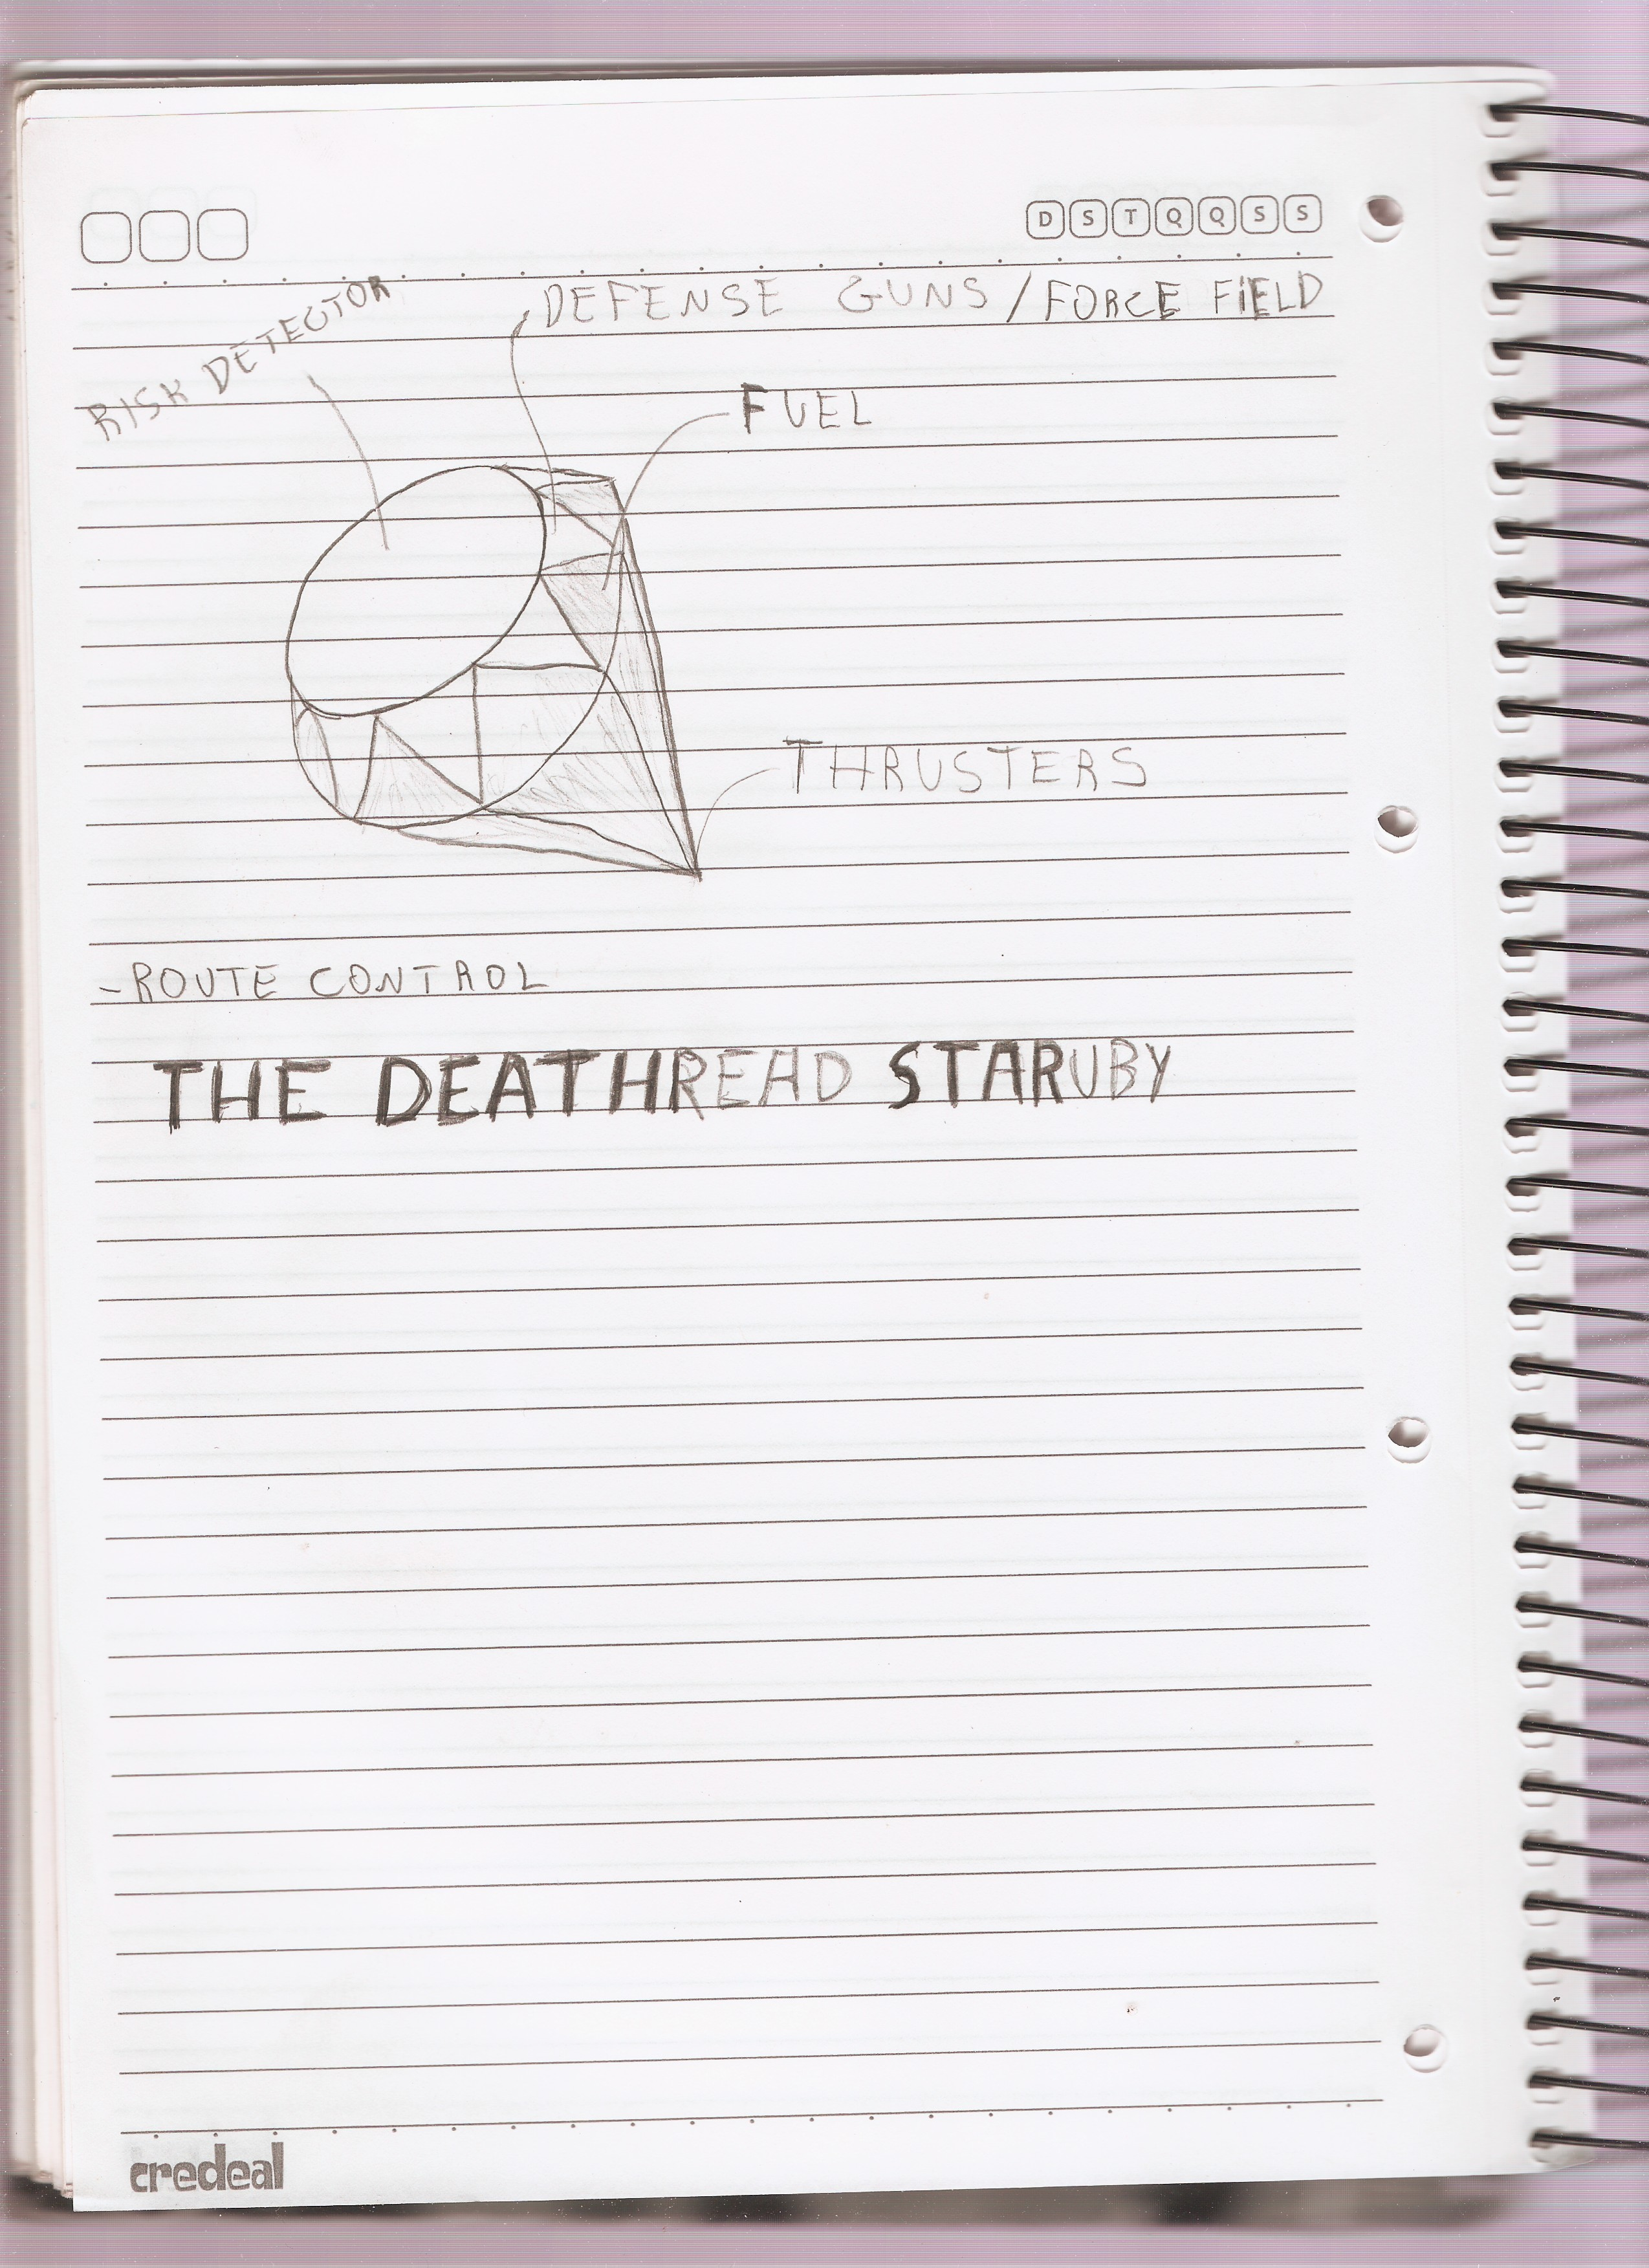
\includegraphics[scale=0.1]{slides/DEATHread-STARuby.jpg}
	\end{figure}
\end{frame}



\section{Introdução}

	\subsection{Problema escolhido}
%----------------------------------------------------------------------------%

	\begin{frame}
	\frametitle{Problema escolhido}
		 \begin{block}{}
				O problema escolhido é um simulador simples destinado a, obviamente, simular uma nave espacial em viajem. Os recursos principais da nave são separados em módulos, e cada módulo é executado por uma Thread.
		 \end{block}
	\end{frame}

	\subsection{Contexto}
	\begin{frame}
	\frametitle{Contexto}
		 \begin{block}{}
				\begin{itemize}
			    \item A nave possui uma classe que representa um sensor, com o status de recursos como energia, combustivel e dano.
					\pause
					\item Ao inicial a nave, os módulos são ligados, e cada Thread que representa a execução de um módulo começa a ser executada.
				\end{itemize}
		 \end{block}
	\end{frame}

\section{Threads no problema?}
	\subsection{Sobre Threads}
	\begin{frame}
	\frametitle{Por que usar Threads no problema?}
		 \begin{block}{}
		    Os modulos precisam notificar ao sensor o quanto estão gastando de recursos, ou se a nave recebeu algum dano, e aí se encontra a solução pelas Threads, já que todos devem notificar os sensores de forma concorrente.
		 \end{block}
	\end{frame}

	\begin{frame}
	\frametitle{Threads: explicações}
		 \begin{block}{}
				As Threads servem para separar a aplicação a ser executada em várias linhas de execução, de forma que estas linhas seja executadas concorrentemente e sincronizadamente.
		 \end{block}
	\end{frame}
	\begin{frame}
	\frametitle{Threads: explicações}
		 \begin{block}{}
				As Threads servem para separar a aplicação a ser executada em várias linhas de execução, de forma que estas linhas seja executadas concorrentemente e sincronizadamente.
		 \end{block}
	\end{frame}

	\subsection{Sobre Threads no ruby}
	\begin{frame}
	\frametitle{Threads no ruby}
		 \begin{block}{}
				No ruby, as Threads  são implementadas a nivel de aplicação, até mesmo porque é a maquina virtual do ruby que vai gerenciar a concorrencia das threads.
		 \end{block}
	\end{frame}

\section{Código principal}
	\subsection{Código principal}
	\begin{frame}
	\frametitle{Pseudo Código principal}
		 \begin{block}{}
				Como foi visto no  pseudocódigo, foi nescessário sincronizar o acesso aos sensores. Já que todos os modulos vão notificar os sensores concorrentemente, se isso não for sincronizado, dados não consistentes poderão ser colocados nos sensores.
		 \end{block}
	\end{frame}

	\begin{frame}
	\frametitle{Sobre o sistema}
		 \begin{block}{}
				Para tornar a notificação dos sensores Thread-safe (poder ser chamado por diversas threads sem causar inconsistencia nos dados), foi necessário implementar um semáforo em que cada thread passa por esse semáforo para notificar os sensores.
		 \end{block}
	\end{frame}

	\begin{frame}
	\frametitle{Sobre o sistema}
		 \begin{block}{}
				Para tornar a notificação dos sensores Thread-safe (poder ser chamado por diversas threads sem causar inconsistencia nos dados), foi necessário implementar um semáforo em que cada thread passa por esse semáforo para notificar os sensores.
		 \end{block}
	\end{frame}

	\begin{frame}
	\frametitle{Sobre o sistema}
		 \begin{block}{}
				O semáforo no caso, é uma classe chamada Mutex (mutual exclusion). Sendo assim, é criada uma instancia da classe Mutex, e essa instancia é chamada por cada Thread para sincronizar a parte devida do codigo.
		 \end{block}
	\end{frame}

	\section{Desenvolvimento}
	\subsection{Desenvolvimento}
	\begin{frame}
	\frametitle{Desenvolvimento}
		 \begin{block}{}
				O desenvolvimento foi feito na maior parte do tempo remotamente, compartilhando o espaço de desenvolvimento por meio de um repositorio no github,  com debates via messenger.
		 \end{block}
	\end{frame}

	\begin{frame}
	\frametitle{Sobre o sistema}
		 \begin{block}{}
				Os testes foram feitos basicamente por testes de unidade, assim, a cada classe criada, era testado a classe individualmente, e,  só posteriormente, integrar as classes para executar o problema.
		 \end{block}
	\end{frame}

	\section{Conclusão}
	\begin{frame}
	\frametitle{Conclusão}
		 \begin{block}{}
				O uso de Threads demonstrou algumas dificuldades, como por exemplo, entender como a maquina virtual faz a concorrencia das Threads; foi visto, por exemplo, que ao chamar uma Thread pelo metodo “run”, a aplicação não executa nenhuma outra Thread enquanto a execução desta não terminar, sendo nescessário usar o método “join” para repartir o tempo da CPU para diversas Threads que estão executando loops.
		 \end{block}
	\end{frame}



%\begin{frame}[allowframeworks] 
   \frametitle{Referências Bibliográficas}
   \bibliography{bibliography/apresentacao}
   \bibliographystyle{plain}
\end{frame}


\end{document}


